\section{Hardware empleado en el proyecto}
Con el fin de obtener una vista general de todo el proyecto, así como del coste del mismo se lista a continuación todos los componentes del robot y su coste:
\begin{itemize}
	\item Chasis del vehículo. Fabricado a partir de un tablón plano de edf cortado en una cnc láser de forma gratuita gracias al Fablab de la Universidad de Sevilla en la facultad de Arquitectura.
	\item Motores de corriente continua(~1pavos). Adquiridos a través de tiendas digitales por un módico precio, lo cual se refleja en una calidad más bien pésima. Sin embargo, formaban parte de un kit que incluye ruedas y acople al eje de transmisión, suponiendo un ahorro importante de tiempo y dinero. 
	\item Encoders ópticos (~6pavos). Compuestos por un diodo emisor de luz comprados también a través de internet y por un disco que interrumpe el paso del haz lumínico diseñado específicamente e impreso en 3D.
	\item Microcontrolador ATmega328 (~10pavos). Aunque la gran parte del código implementado en el micro no utiliza las librerías de arduino, por comodidad se ha optado por un microchip ya montado en una placa tipo arduino (un modelo no oficial, clónico).
	\item IMU mpu-6050 (~2pavos).
	\item Raspberry Pi 3B+ (~30pavos). Constituye el cerebro del robot, y centraliza la comunicación con los demás sistemas. Aunque puede resultar el componente más caro del proyecto, se disponían de varias de antemano, por lo que no hubo que asumir su coste.
	\item Kinect for Xbox 360 de Microsoft (~15pavos). Esta popular cámara merece la fama que tiene por lo asequible que es (especialmente el modelo más antiguo) y las utilidades que trae. Se demuestra como la opción más socorrida para desarollar con poco presupuesto aplicaciones que requieran de imágenes o sensores de profundidad.
	
\end{itemize}
\subsection{Estructura}
El robot ha sido diseñado con una topología inspirada en los vehículos de exploración espacial conocidos como \textit{rovers}, utilizando materiales y métodos de construcción asequibles y manteniendo como objetivo una sencilla sustitución e iterabilidad de cada componente. La estructura está diseñada en \textit{FreeCad} y compuesta por piezas de madera mecanizadas en una cortadora láser cnc.
Algunos elementos sin funcionalidad estructural, como los encoders o el soporte de la cámara, han sido fabricados mediante impresión 3D.
\begin{figure}[h!]
	\centering
	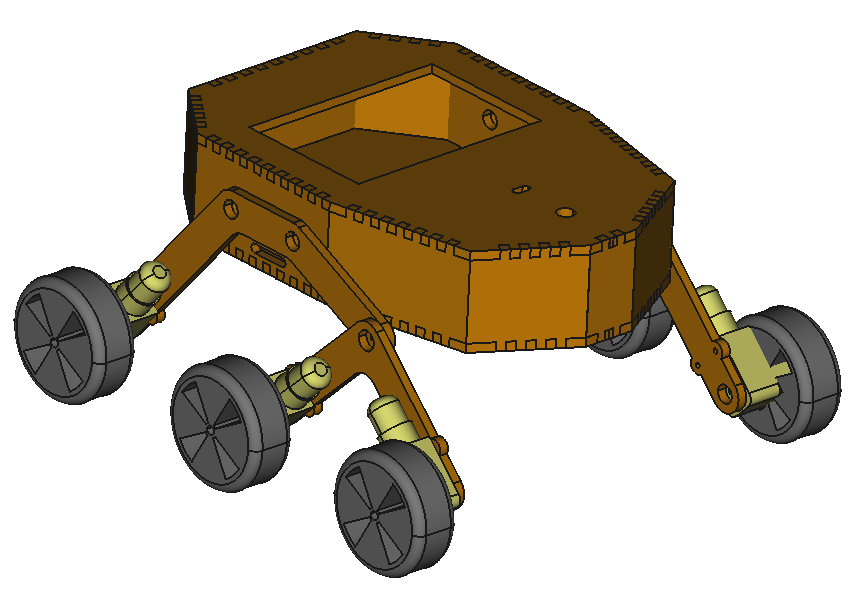
\includegraphics[width=.6\textwidth]{images/wheele_stl}
	\caption{Modelo CAD del robot}
\end{figure}
\\
La disposición geométrica es la de un vehículo diferencial, con tres pares de ruedas, cada una con su respectiva pareja de motor y encoder.\\
\subsection{Diseño PCB}
\subsection{Controladores de abordo}
\subsubsection{Raspberry Pi}
\subsubsection{Arduino}
\subsection{Cámaras empleadas}